%; whizzy paragraph -pdf xpdf -latex ./whizzypdfptex.sh
%; whizzy-paragraph "^\\\\begin{frame}\\|\\\\emtext"
% latex beamer presentation.
% platex, latex-beamer $B$G%3%s%Q%$%k$9$k$3$H$rA[Dj!#(B 

%     Tokyo Debian Meeting resources
%     Copyright (C) 2012 Junichi Uekawa

%     This program is free software; you can redistribute it and/or modify
%     it under the terms of the GNU General Public License as published by
%     the Free Software Foundation; either version 2 of the License, or
%     (at your option) any later version.

%     This program is distributed in the hope that it will be useful,
%     but WITHOUT ANY WARRANTY; without even the implied warreanty of
%     MERCHANTABILITY or FITNESS FOR A PARTICULAR PURPOSE.  See the
%     GNU General Public License for more details.
%     You should have received a copy of the GNU General Public License
%     along with this program; if not, write to the Free Software
%     Foundation, Inc., 51 Franklin St, Fifth Floor, Boston, MA  02110-1301 USA

\documentclass[cjk,dvipdfmx,12pt]{beamer}
\usetheme{Tokyo}
\usepackage{monthlypresentation}

%  preview (shell-command (concat "evince " (replace-regexp-in-string "tex$" "pdf"(buffer-file-name)) "&")) 
%  presentation (shell-command (concat "xpdf -fullscreen " (replace-regexp-in-string "tex$" "pdf"(buffer-file-name)) "&"))
%  presentation (shell-command (concat "evince " (replace-regexp-in-string "tex$" "pdf"(buffer-file-name)) "&"))

%http://www.naney.org/diki/dk/hyperref.html
%$BF|K\8l(BEUC$B7O4D6-$N;~(B
\AtBeginDvi{\special{pdf:tounicode EUC-UCS2}}
%$B%7%U%H(BJIS$B7O4D6-$N;~(B
%\AtBeginDvi{\special{pdf:tounicode 90ms-RKSJ-UCS2}}

\newenvironment{commandlinesmall}%
{\VerbatimEnvironment
  \begin{Sbox}\begin{minipage}{1.0\hsize}\begin{fontsize}{8}{8} \begin{BVerbatim}}%
{\end{BVerbatim}\end{fontsize}\end{minipage}\end{Sbox}
  \setlength{\fboxsep}{8pt}
% start on a new paragraph

\vspace{6pt}% skip before
\fcolorbox{dancerdarkblue}{dancerlightblue}{\TheSbox}

\vspace{6pt}% skip after
}
%end of commandlinesmall

\title{$B=i$a$F$N%-!<%5%$%s%Q!<%F%#(B}
\author{$Bc7F#(B $BM:2p(B  ysaito@golangcoder.club}
\date{2017$BG/(B9$B7n(B16$BF|(B}
\logo{
\includegraphics[width=8cm]{image200607/openlogo-light.eps}}

\begin{document}

\begin{frame}
\titlepage{}
\end{frame}

\begin{frame}{$B;29M$K$7$?;qNA(B}
  $B%-!<%5%$%s%Q!<%F%#$G;29M$K$5$;$F$$$?$@$$$?;qNA(B

  %%BoundingBox: 0.00 0.00 362.83 272.13
  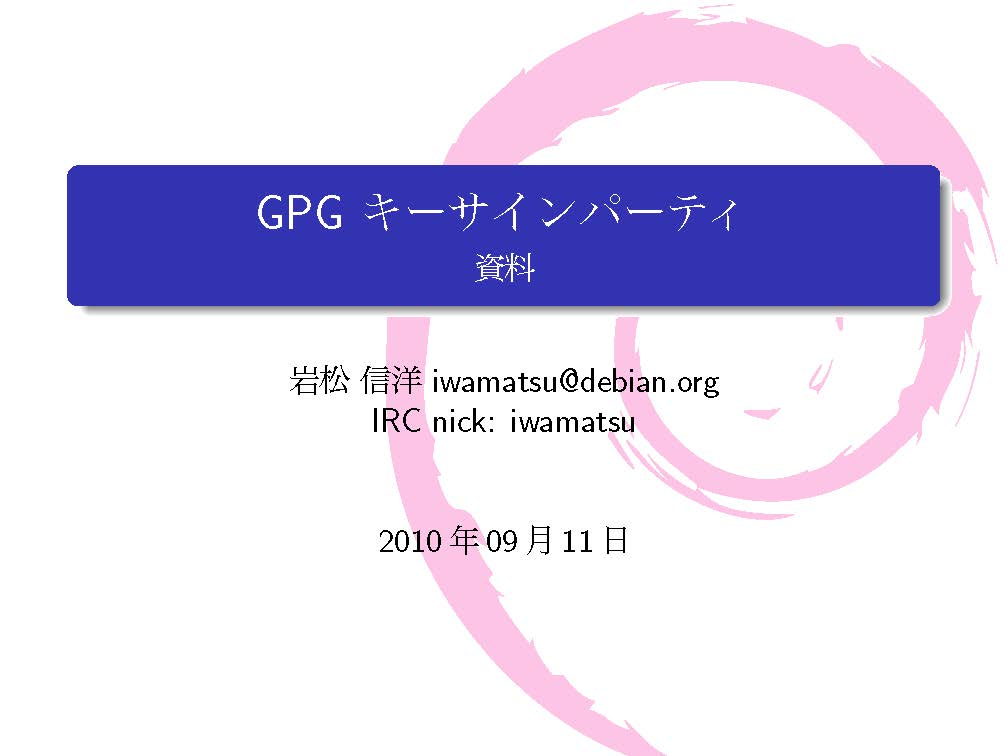
\includegraphics[width=0.8\hsize]{image201709/shiryo001.jpg}
  \end{frame}


\section{}
%\emtext{}

\begin{frame}[containsverbatim]{caff$B$r;H$*$&$H$7$F(B}
Homebrew $B$+$i>C$($F$?(B
\begin{commandline}
$ brew search signing-party
 ==> Searching local taps...
 ==> Searching taps on GitHub...
 ==> Searching blacklisted, migrated and deleted formulae...
 signing-party was deleted from homebrew/core in commit e05298ad8a:
\end{commandline}
\end{frame}

\begin{frame}{gpg$B$N$_$G$d$C$F$_$h$&(B}
  %%BoundingBox: 0.00 0.00 362.83 272.13
  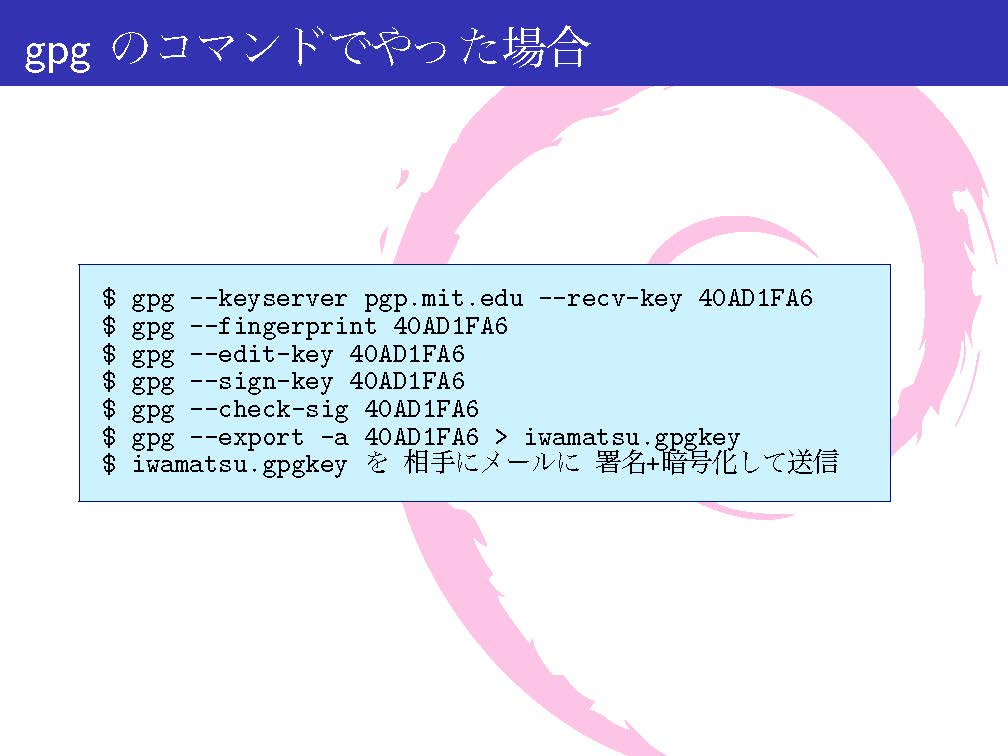
\includegraphics[width=0.8\hsize]{image201709/shiryo002.jpg}
\end{frame}

\begin{frame}[fragile]{$B$D$^$E$$$?(B}
$BAj<j$N8x3+80$G0E9f2=$9$k$H$3$m$r<+J,$N8x3+80$G0E9f2=$7$F$7$^$C$?(B
\begin{commandline}
$ gpg --encrypt --recipient $BAj<j$N8x3+80(BID $BAj<j$N8x3+80(B
\end{commandline}
  %%BoundingBox: 0.00 0.00 362.83 272.13
  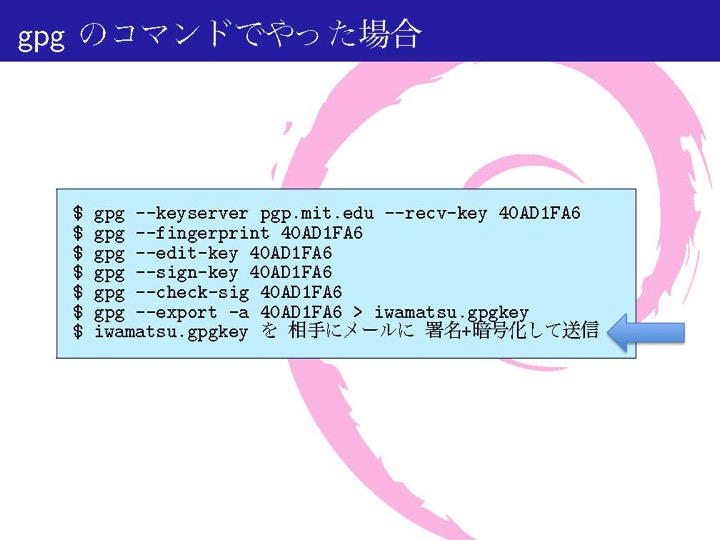
\includegraphics[width=0.8\hsize]{image201709/shiryo003.jpg}
\end{frame}

\begin{frame}[containsverbatim]{caff$B$r$D$+$o$J$$$J$i(B}
$B;29M(B: https://github.com/thinkAmi/caffish-ps
\begin{commandline}
# $B%-!<%5!<%P$h$jAj<j$N8x3+80$r<hF@$7!"(B
# $B<+J,$N8x3+80$N80B+$KF~$l$k(B
$ gpg --keyserver pgp.mit.edu --recv-key $BAj<j$N8x3+80(BID

# $BI=<($5$l$k%U%#%s%,!<%W%j%s%H$H!"(B
# $B<j85$N=qN`$N%U%#%s%,!<%W%j%s%H$,0lCW$7$F$$$k$3$H$r3NG'(B
$ gpg --fingerprint $BAj<j$N8x3+80(BID

# $BAj<j$N8x3+80$K=pL>(B
$ gpg --sign-key $BAj<j$N8x3+80(BID

# $B=pL>$7$?8x3+80$r%(%/%9%]!<%H(B
$ gpg --export -a $BAj<j$N8x3+80(BID > ./foo.gpgkey

# $B<+J,$NHkL)80$G=pL>$7$?Aj<j$N8x3+80$r!"Aj<j$N8x3+80$r;H$C$F0E9f2=(B
$ gpg --no-auto-check-trustdb  --trust-model=always \
  --armor --recipient $BAj<j$N8x3+80(BID --encrypt ./foo.gpgkey
# foo.gpgkey.asc $B$,@8@.$5$l$k(B
# $B0E9f2=$7$?8x3+80$r%a!<%k$KE:IU$7!"(B
# $B%a!<%kK\J8$r0E9f2=$7$FAj<j$XAw?.(B
\end{commandline}
\end{frame}

\begin{frame}
\Huge $B$=$&$@(B caff $B$D$+$*$&(B 
\end{frame}

\begin{frame}[fragile]{$B$b$&0l$D5M$^$C$?$H$3$m(B}
  Debian strech $B$K(B caff $B$r$$$l$F(B
  $B%a!<%k%5!<%P$rN)$F$F(B...
  \begin{commandline}
$ caff -u $B<+J,$N8x3+80(BID $B0l?ML\$N8x3+80(BID $BFs?ML\$N8x3+80(BID...
[NOTICE] Fetching keys from pool.sks-keyservers.net, this may take a while...
[WARN] Local-user $B<+J,$N8x3+80(BID is not defined as one of your keyid in ~/.caffrc (it will not be used)
[ERROR] None of the local-user keys seem to be known as a keyid listed in ~/.caffrc
# ~/.caffrc $B$O$A$c$s$H@_Dj$7$F$$$k$O$:$@$1$I(B...
# $B<+J,$N8x3+80$N%U%#%s%,!<%W%j%s%H$N8eH>#1#67e(B

$ caff $B0l?ML\$N8x3+80(BID $BFs?ML\$N8x3+80(BID...
# $BDL$C$?(B
  \end{commandline}
  
\end{frame}

\end{document}

;;; Local Variables: ***
;;; outline-regexp: "\\([ 	]*\\\\\\(documentstyle\\|documentclass\\|emtext\\|section\\|begin{frame}\\)\\*?[ 	]*[[{]\\|[]+\\)" ***
;;; End: ***

